%!TEX root = ../main.tex

\section{Mass fit (5 pages)}
\label{sec:b02dd:massfit}

In this section, the fit of the invariant $m_{\Dp\Dm}$ mass distribution is
described which is used to calculate signal candidates weights via the \SPlot
method and thereby discriminates between signal and background candidates. As
the linear Pearson correlation coefficient between the invariant mass and the
decay time is determined to be $\rho = \num{0.007}$ it is valid to apply the
sWeights in the decay time fit later on (see \cref{sec:b02dd:decaytimefit}) to
obtain the \CP observables.

The mass distribution is parametrized with a \PDF $\mathcal{P}$ consisting of
five components, \BdToDD signal, \BsToDD background, background from \BdToDsD,
background from \BsToDsD, and combinatorial background:
%
\begin{equation}
\resizebox{0.9\textwidth}{!}{$
  N^s \mathcal{P}^s = \yield{$s$}{\Bd} \pdf{$s$}{\Bd} + \yield{$s$}{\Bs} \pdf{$s$}{\Bs} + \yield{$s$}{\BdToDsD} \pdf{$s$}{\BdToDsD} + \yield{$s$}{\BsToDsD} \pdf{$s$}{\BsToDsD} + \yield{$s$}{Bkg} \pdf{$s$}{Bkg}$ \, .}
\end{equation}
%
In the extended maximum likelihood fit four disjoint categories are
simultaneously fitted. It is distinguished between the two years of
data-taking 2011 and 2012 and between the two final states $\KpipiKpipi$ and
$\KKpiKpipi$ ($s = \{2011,\Kpipi\}, \{2011, \KKpi\}, \{2012, \Kpipi\}, \{2012,
\KKpi\}$). The tagging output is not split.

\paragraph{$\boldsymbol{\BdToDD}$ signal:}
The $\BdToDD$ signal mass component is modelled by the sum of three Crystal
Ball functions~\cite{Skwarnicki:1986xj} which share a common peak position
$\mu_{\Bd}$ but have different width parameters $\sigma_i$. Two of the Crystal
Ball functions have a tail towards lower masses and one has a tail towards
higher masses. The parameters $\alpha_1$ to $\alpha_3$ of the power law
functions, the ratio between the widths, and the fractions $f_1$ and $f_2$
between the Crystal Ball functions are determined from a fit to the invariant
$\Dp\Dm$ mass distribution of $\BdToDD$ signal MC in the range
\SIrange{4800}{5400}{\MeVcc}. This MC sample consists of both final states
generated in the ratio of the current world averages~\cite{PDG2014}. Apart
from the mass range the full selection is applied. The background categories
\num{0}, \ie \texttt{Signal}, and \num{50}, \ie \texttt{LowMassBkg} with
missing photons, are considered. Events of the latter category create a very
long tail towards lower masses which require the third Crystal Ball function.
The fit results are listed in \cref{tab:b02dd:massfit:mc_fitresults} and a
plot of the distribution overlaid with the projection of the PDF is given in
\cref{fig:b02dd:massfit:mc}.
%
\begin{table}[!htb]
\centering
\caption{Fit results of the mass fit to \BdToDD signal MC.}%
\label{tab:b02dd:massfit:mc_fitresults}
\begin{tabular}{llr@{$\,\pm\,$}l}
  \toprule
  \multicolumn{2}{c}{Parameter}                   & \multicolumn{2}{c}{Value}  \\
  \midrule
  $\param{\mu}{MC}{\Bd}$    & ($\si{MeV/c^{2}}$)  & $5279.70$    & $0.09$      \\
  $\param{\sigma}{MC}{1}$   & ($\si{MeV/c^{2}}$)  & $8.5$        & $0.4$       \\
  $\param{\sigma}{MC}{2}$   & ($\si{MeV/c^{2}}$)  & $16$         & $5$         \\
  $\param{\sigma}{MC}{3}$   & ($\si{MeV/c^{2}}$)  & $9.0$        & $0.4$       \\
  $\param{f}{MC}{1}$        &                     & $0.48$       & $0.06$      \\
  $\param{f}{MC}{2}$        &                     & $0.0098$     & $0.0011$    \\
  $\param{\alpha}{MC}{1}$   &                     & $1.18$       & $0.08$      \\
  $\param{\alpha}{MC}{2}$   &                     & $0.12$       & $0.04$      \\
  $\param{\alpha}{MC}{3}$   &                     & $-1.46$      & $0.08$      \\
  \bottomrule
\end{tabular}
\end{table}
%
\begin{figure}[!htb]
\centering
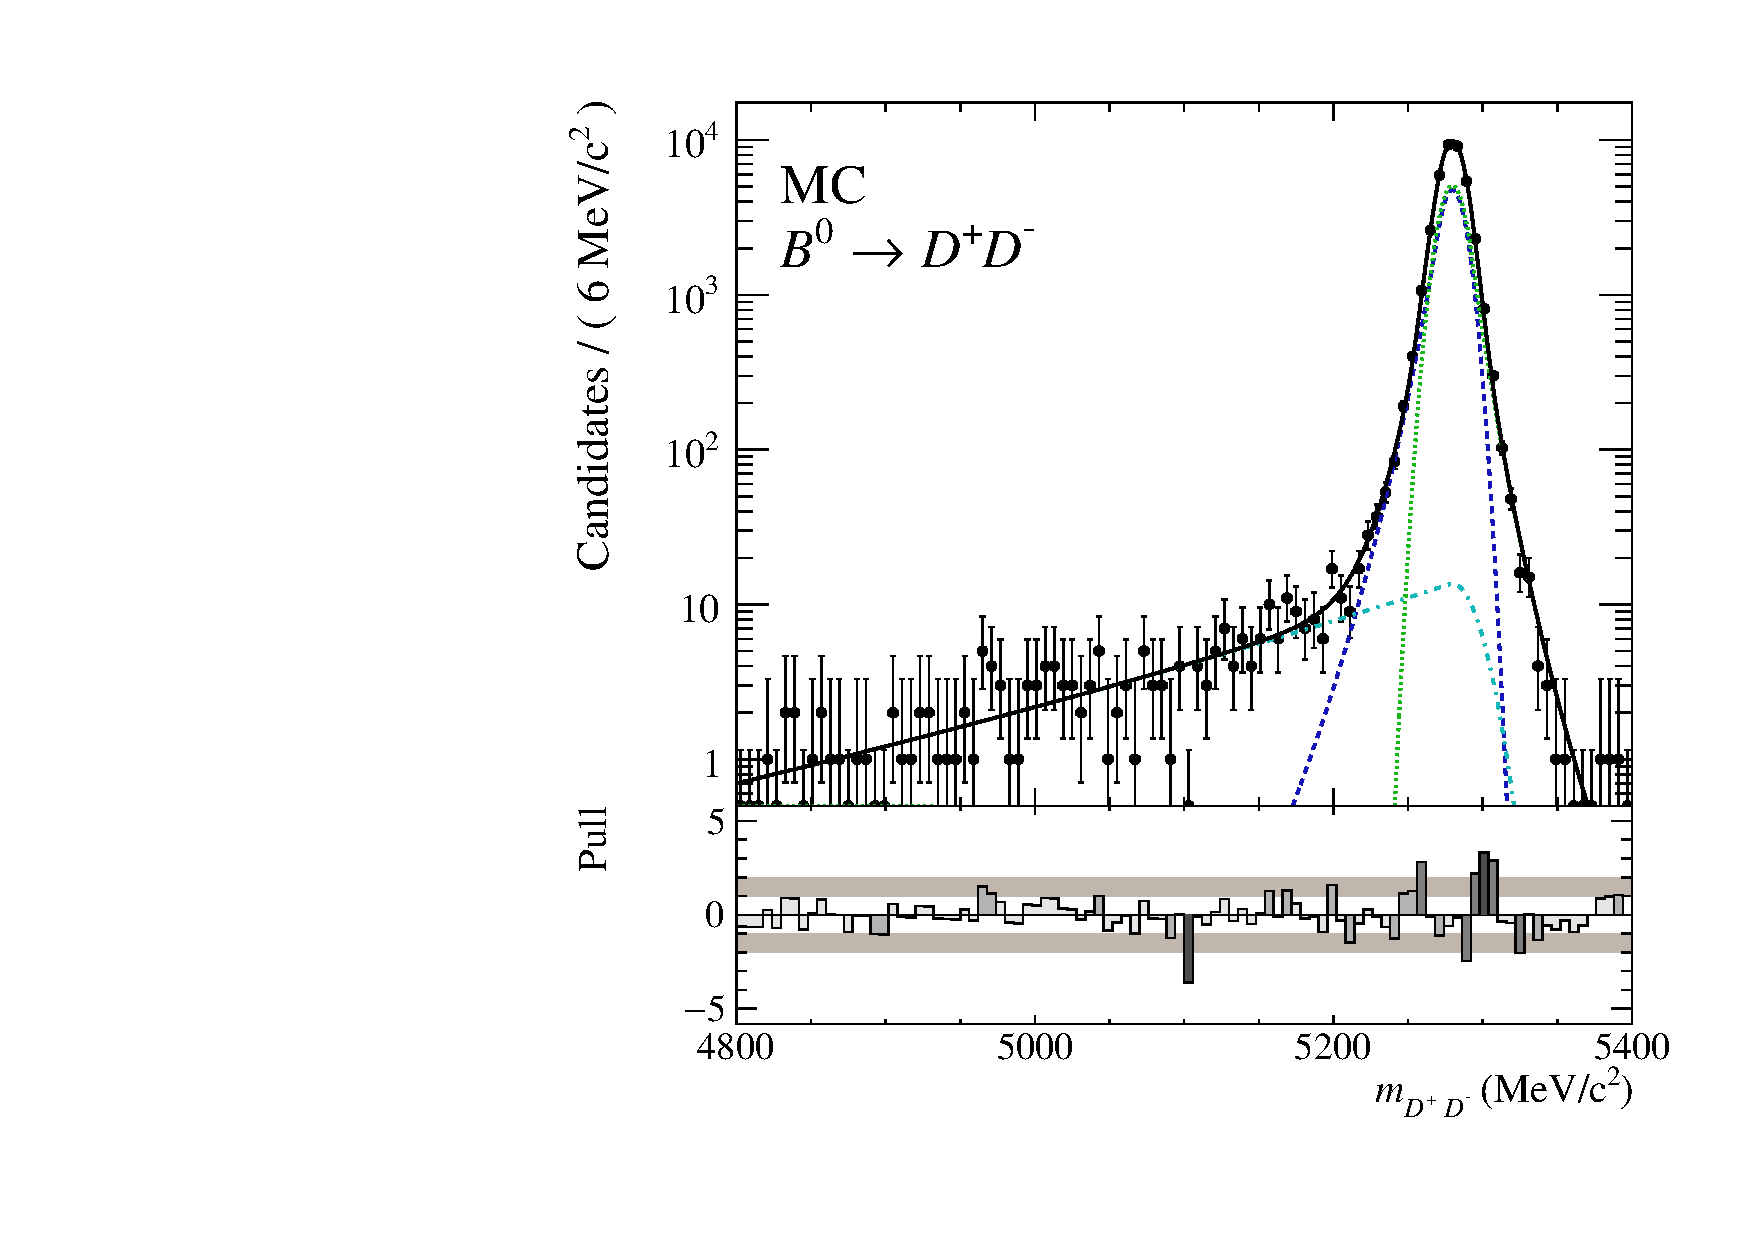
\includegraphics[width=0.49\textwidth]{07-B02DD/figs/obsMass_MC.pdf}
\caption{Mass distribution of the \BdToDD signal MC sample overlaid with the
projection of the fitted PDF. The y-axis has a logarithmic scale.}%
\label{fig:b02dd:massfit:mc}
\end{figure}
%
The exponent $n$ of all power law parts is fixed to \num{10}. The widths
$\param{\sigma}{MC}{1}$ to $\param{\sigma}{MC}{3}$ are multiplied by a common
scale factor $R$ in the fit to data to account for differences in the mass
resolution between simulation and data.

\paragraph{$\boldsymbol{\BsToDD}$ background:}
Apart from the $\Bd$ also the heavier $\Bs$ can decay to the $\Dp\Dm$ final state.
Almost the same parametrization as for the $\Bd$ signal component is used, \ie
same width and tail parameters, while the peak position is shifted by the
world average $\dmBdBs = \mu_{\Bs} - \mu_{\Bd} =
\SI{87.35}{\MeVcc}$~\cite{PDG2014}.

\paragraph{$\boldsymbol{\BdToDsD}$ background:}
The vetoes applied in the selection suppress the contribution from
misidentified kaons. Nevertheless, a significant amount of $\BdToDsD$ decays
remains in the data sample. A sum of two Crystal Ball PDFs is used to
parametrize their invariant mass distribution. The fraction parameter and the tail
parameters are determined from a fit to the invariant mass distribution of
simulated $\BdToDsD$ events reconstructed as $\BdToDD$. Again, the full
selection is applied as this could change the shape. The fit results are listed in
\cref{tab:massfit:DsDMC} and the corresponding plot is shown in
\cref{fig:massfit:DsDMC}.
%
\begin{table}[!htb]
\centering
\caption{Fit results of the mass fit to \BdToDsD MC.}
\label{tab:massfit:DsDMC}
\begin{tabular}{llr@{$\,\pm\,$}l}
  \toprule
  \multicolumn{2}{c}{Parameter}                        & \multicolumn{2}{c}{Value} \\
  \midrule
  $\param{\mu}{MC}{\BdToDsD}$    & ($\si{MeV/c^{2}}$)  & $5222.2$    & $0.9$       \\
  $\param{\sigma}{MC}{1,\DsD}$   & ($\si{MeV/c^{2}}$)  & $15.0$      & $1.5$       \\
  $\param{\sigma}{MC}{2,\DsD}$   & ($\si{MeV/c^{2}}$)  & $20.7$      & $2.1$       \\
  $\param{f}{MC}{1,\DsD}$        &                     & $0.78$      & $0.13$      \\
  $\param{\alpha}{MC}{1,\DsD}$   &                     & $0.60$      & $0.09$      \\
  $\param{\alpha}{MC}{2,\DsD}$   &                     & $-1.8$      & $0.4$       \\
  \bottomrule
\end{tabular}
\end{table}
\begin{figure}
\centering
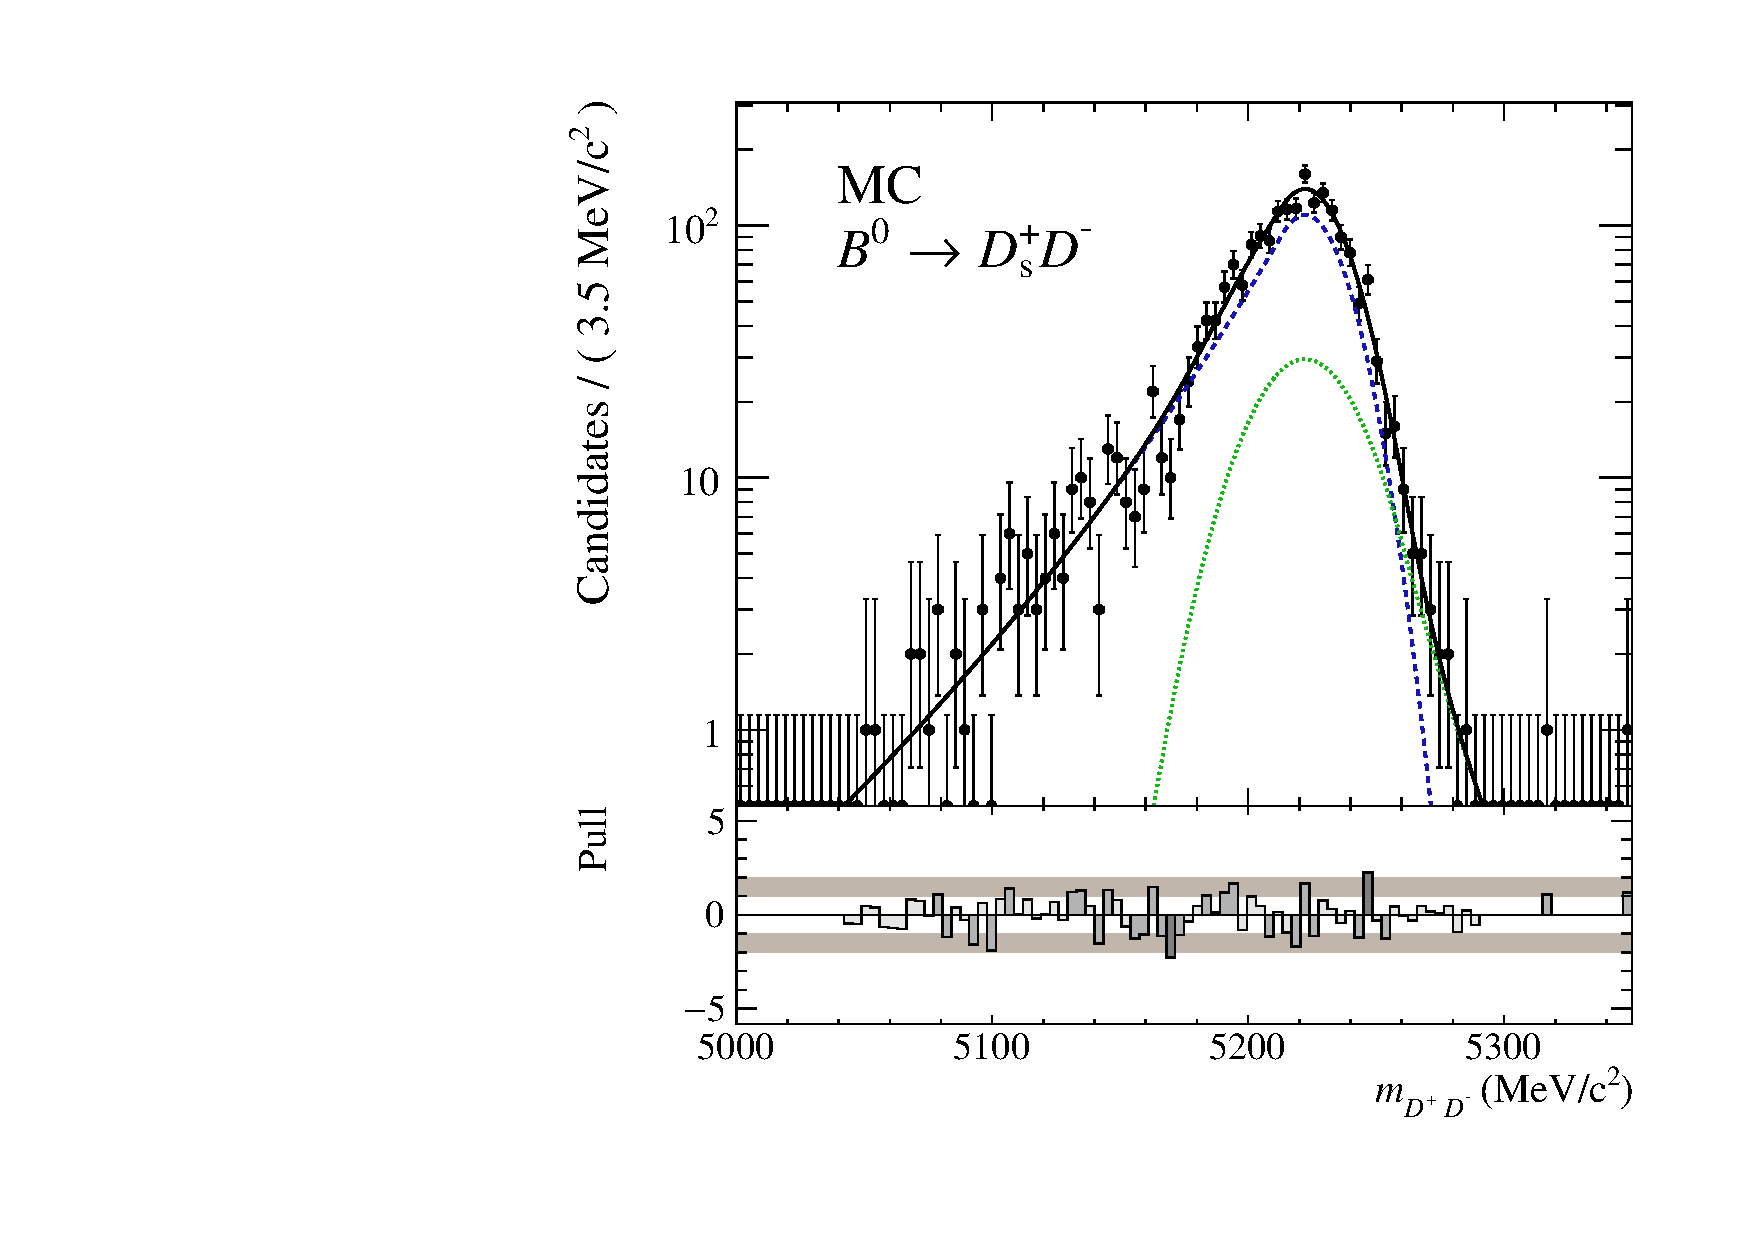
\includegraphics[width=0.49\textwidth]{07-B02DD/figs/DsDMass_MC.pdf}
\caption{Mass distribution of the $\BdToDsD$ MC sample reconstructed as
$\BdToDD$ overlaid with the projection of the two Crystal Ball PDFs. The
y-axis has a logarithmic scale.}
\label{fig:massfit:DsDMC}
\end{figure}
%
The power law exponent $n$ is fixed to \num{10}. The width parameters as well
as the peak position are floating parameters in the fit to data.

\paragraph{$\boldsymbol{\BsToDsD}$ background:}
Although only few candidates of $\BsToDsD$ decays are expected this contribution is
included in the nominal fit. Like the $\Bd$ component it is parametrized with
the sum of two Crystal Ball PDFs. The peak position is constrained to the sum
of the peak position of the $\Bd$ component and the mass difference $\dmBdBs$. All
other shape parameters are shared with the ones for the $\Bd$ component.

\paragraph{Combinatorial background:}
The reconstructed mass PDF of the combinatorial background is modelled by an
exponential function with individual slopes
$\param{\beta}{\Kpipi}{}$ and $\param{\beta}{\KKpi}{}$ based on the number of
kaons in the final state.

\bigskip\noindent
In \cref{tab:b02dd:FitResultsMass} the results of the floating shape
parameters of the mass fit to data are shown.
%
\begin{table}[!htb]
\centering
\caption{Results of the floating shape parameters in the mass fit to data.}
\label{tab:b02dd:FitResultsMass}
\centering
\begin{tabular}{llr@{$\,\pm\,$}l}
  \toprule
  \multicolumn{2}{c}{Parameter}                                & \multicolumn{2}{c}{Value}  \\
  \midrule
  $\param{\mu}{}{\Bd}$           & ($\si{MeV/c^{2}}$)          & $5279.26$    & $0.29$      \\
  $\param{R}{}{\Bd}$             &                             & $0.995$      & $0.032$     \\
  \midrule
  $\param{\mu}{}{\DsD}$          & ($\si{MeV/c^{2}}$)          & $5218.2$     & $1.1$       \\
  $\param{\sigma}{}{1,\DsD}$     & ($\si{MeV/c^{2}}$)          & $19.2$       & $2.7$       \\
  $\param{\sigma}{}{2,\DsD}$     & ($\si{MeV/c^{2}}$)          & $14.3$       & $3.1$       \\
  $\param{\beta}{}{\KpipiKpipi}$ & ($\si{1/(MeV/c^{2}})$)      & $-0.0031$    & $0.0005$    \\
  $\param{\beta}{}{\KKpiKpipi}$  & ($\si{1/(MeV/c^{2}})$)      & $-0.0041$    & $0.0006$    \\
  \bottomrule
\end{tabular}
\end{table}
%
The $\Bd$ peak position is in good agreement with the world average of
$\param{\mu}{WA}{\Bd} = \SI{5279.58\pm0.17}{\MeVcc}$~\cite{HFAG}. The scale
factor $R$ is compatible with unity which means that the mass resolution of
the signal component is well simulated. The slopes of the combinatorial
background differ significantly between the two subsamples showing the benefit
of splitting them to achieve an improved mass description. In
\cref{fig:massfit} the complete data-sample is plotted overlaid with the PDF
projections and its components.
%
\begin{figure}[!htb]
\centering
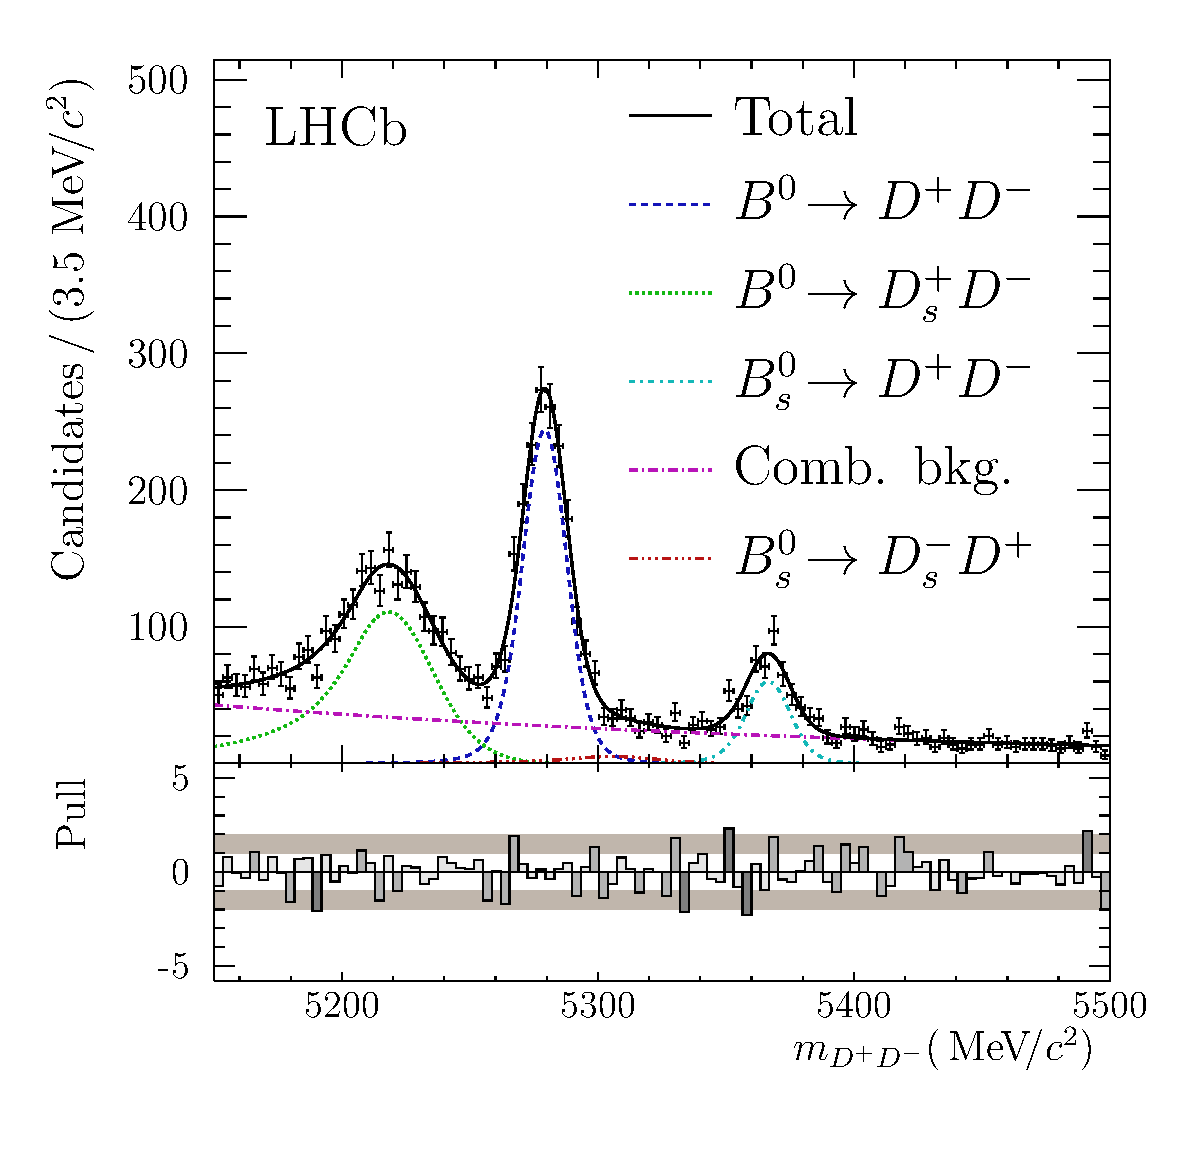
\includegraphics[width=0.5\textwidth]{07-B02DD/tikz/pdf/obsMass_summed_pull.pdf}
\caption{Plot of the reconstructed mass of the \BdToDD data sample with the
projected \PDF and pull distribution.
% Besides the data points and the full \PDF (solid black) the projections of the
% \Bd signal (dashed blue), the \BsToDD background (short-dash-dotted
% turquoise), the \BdToDsD background (dotted green), the \BsToDsD background
% (long-dash- three-dotted red) and the combinatorial background
% (long-dash-dotted purple) are shown.
}
\label{fig:massfit}
\end{figure}
%
The total number of $\Bd$ signal candidates is $N_{\Bd}$ = \num{1610\pm50}.
From the two times higher integrated luminosity and the increased production
cross-section which in first order scales with the centre-of-mass energies
(8/7) one expects \num{2.3} times more signal candidates in the 2012 subsample
than in the 2011 subsample and this can indeed be observed for the fitted
yields. Additionally, there are around five times more signal candidates in
the final state with two kaons than with three kaons which also meets the
ecpectations from the branching ratios.

\FloatBarrier